% Manufactured Death: Mathematical Modeling of HIV Prevention Impossibility
% Among People Who Inject Drugs
% Formatted for The Lancet HIV
% Last updated: December 26, 2025

\documentclass[11pt]{article}

% Lancet HIV formatting requirements
\usepackage[margin=1in]{geometry}
\usepackage{times}
\usepackage{setspace}
\usepackage{graphicx}
\usepackage{booktabs}
\usepackage{amsmath}
\usepackage{amssymb}
\usepackage[numbers,super,sort&compress]{natbib}
\usepackage{url}
\usepackage{hyperref}
\usepackage{xcolor}
\usepackage{lineno}
\usepackage{caption}

% Lancet style settings
\doublespacing
\linenumbers
\captionsetup{labelfont=bf,font=small}

% Custom commands
\newcommand{\Rzero}{R$_0$}

\begin{document}

% TITLE PAGE
\begin{center}
{\Large\bfseries Manufactured Death: Mathematical Modeling of HIV Prevention Impossibility Among People Who Inject Drugs}

\vspace{0.5cm}

{\large\itshape A Barrier Decomposition Analysis}

\vspace{1cm}

AC Demidont, MD$^{1}$

\vspace{0.5cm}

$^1$Nyx Dynamics LLC

\vspace{0.5cm}

\textbf{Correspondence to:}\\
AC Demidont, MD\\
Nyx Dynamics LLC\\
Email: research@nyxdynamics.com

\vspace{1cm}

\textbf{Word count:} 3,847 (excluding abstract, tables, figures, references)\\
\textbf{Abstract word count:} 298\\
\textbf{Tables:} 2\\
\textbf{Figures:} 5\\
\textbf{References:} 45
\end{center}

\newpage

% ABSTRACT
\section*{Abstract}

\textbf{Background:} HIV prevention among the 15.6 million people who inject drugs (PWID) globally has relied primarily on stochastic avoidance---probability-based prevention rather than systematic intervention. We hypothesized that nested barriers create a mathematical impossibility of achieving the sustained protection state (\Rzero{}=0) necessary for epidemic control, regardless of pharmacological efficacy.

\textbf{Methods:} We developed a three-layer barrier framework decomposing HIV prevention failure into: (1) Pathogen Biology---rapid establishment of irreversible \Rzero{}>0; (2) HIV Testing Failures---inadequate acute infection detection; and (3) Architectural Failures---policy, stigma, infrastructure, research exclusion, and algorithmic barriers. Monte Carlo simulation (n=100,000 per scenario) quantified cascade completion probability for long-acting injectable pre-exposure prophylaxis (LAI-PrEP) implementation across eight policy scenarios. A stochastic avoidance failure model predicted outbreak probability incorporating methamphetamine prevalence trajectories and network density evolution.

\textbf{Findings:} Under current policy, P(\Rzero{}=0) = 0.00\% (95\% CI: 0.00--0.00) for PWID, compared to 16.30\% for men who have sex with men (MSM) receiving identical pharmacological intervention---an infinite-fold disparity. Barrier decomposition attributed 93.2\% to architectural failures (policy 38.4\%, infrastructure 21.9\%, stigma 20.5\%, machine learning 8.2\%, research exclusion 4.1\%), 6.8\% to HIV testing failures, and 0.0\% to pathogen biology. The stochastic avoidance model predicted 63.3\% probability of major outbreak within 5 years (median: 4.0 years). Even with full harm reduction and algorithmic debiasing, maximum achievable P(\Rzero{}=0) was 19.92\%.

\textbf{Interpretation:} HIV prevention failure among PWID is policy-determined, not pharmacology-determined. Current prevention relies on stochastic avoidance, a time-limited phenomenon predicted to fail catastrophically as methamphetamine-driven network density increases. Achieving epidemic control requires fundamental policy change addressing all barrier layers simultaneously.

\textbf{Funding:} None.

\textbf{Keywords:} HIV prevention; people who inject drugs; PrEP; health disparities; mathematical modeling; structural barriers; methamphetamine; implementation science

\newpage

% RESEARCH IN CONTEXT
\section*{Research in Context}

\subsection*{Evidence before this study}
We searched PubMed for articles published from January 1, 2010, to December 1, 2024, using the terms ``HIV prevention,'' ``people who inject drugs,'' ``PrEP,'' ``injection drug use,'' ``structural barriers,'' and ``HIV outbreak.'' Published evidence demonstrates that PWID experience dramatically lower PrEP uptake (0--3\%) compared to MSM (>20\%) despite similar awareness levels. Multiple U.S. outbreaks since 2015 (Scott County, Lawrence/Lowell, Cabell/Kanawha Counties) have occurred in settings with inadequate prevention infrastructure. The Bangkok Tenofovir Study (2013) remains the only major PrEP trial enrolling PWID. Systematic reviews document that criminalization, stigma, and incarceration create barriers to HIV prevention, but no study has quantified the mathematical impossibility of achieving epidemic control under current policy conditions.

\subsection*{Added value of this study}
This study introduces a three-layer barrier framework that quantifies the contribution of pathogen biology (0.0\%), HIV testing failures (6.8\%), and architectural failures (93.2\%) to HIV prevention failure among PWID. We demonstrate that under current policy, the probability of any PWID achieving sustained HIV protection (\Rzero{}=0) is effectively zero---not because of drug efficacy limitations but because of structural barriers functioning as exclusion criteria. The stochastic avoidance failure model provides the first quantitative prediction of outbreak probability (63\% within 5 years) based on methamphetamine prevalence trajectories and network density evolution. The comparison showing identical pharmacological intervention achieving 16.30\% sustained protection in MSM versus 0.00\% in PWID definitively establishes that HIV prevention disparity is policy-determined.

\subsection*{Implications of all the available evidence}
HIV epidemic control among PWID requires simultaneous intervention across all barrier layers. No single policy change can achieve \Rzero{}=0; even theoretical maximum intervention achieves only 19.92\% sustained protection. The 63\% five-year outbreak probability demands urgent action including decriminalization, elimination of healthcare stigma, redesign of prevention infrastructure, mandatory inclusion of PWID in clinical trials, and algorithmic debiasing. Without such changes, future outbreaks are mathematical certainties, not possibilities.

\newpage

% INTRODUCTION
\section{Introduction}

Among the estimated 15.6 million people who inject drugs (PWID) globally, 17.8\% are living with HIV---a prevalence 22 times higher than the general population.\cite{degenhardt_global_2017} Despite three decades of prevention knowledge and pharmacological innovations achieving >99\% efficacy, HIV continues to spread among PWID through mechanisms that current prevention architecture cannot address. We propose that this failure results not from individual behavior or drug efficacy but from nested barriers that create a mathematical impossibility of achieving epidemic control.

The fundamental mathematical requirement for HIV prevention is \Rzero{}=0---sustained protection such that each infected individual transmits to zero others on average. This state requires uninterrupted pharmacological coverage during all potential exposure events. For PWID, achieving \Rzero{}=0 requires not only efficacious drugs but successful navigation of an 8-step prevention cascade: awareness, willingness, healthcare access, disclosure of injection drug use, provider willingness to prescribe, adequate HIV testing, initiation of treatment, and sustained engagement without interruption.

We hypothesized that barriers operating at three distinct levels---pathogen biology, HIV testing algorithms, and architectural failures of the prevention system---create conditions where the product of cascade step probabilities approaches zero, rendering \Rzero{}=0 mathematically unachievable regardless of drug efficacy. This represents a fundamentally different prevention landscape than that faced by men who have sex with men (MSM), where the same pharmacological interventions achieve substantial uptake and sustained protection.\cite{grant_iprex_2010}

Critically, we propose that current HIV ``prevention'' among PWID functions primarily through stochastic avoidance---probability-based prevention where transmission fails to occur due to random chance rather than systematic intervention.\cite{greenhalgh_stochastic_2016,bobashev_firewall_2013} This mechanism is time-limited; as network density increases through methamphetamine-driven behavioral changes and forced geographic clustering, stochastic avoidance will fail catastrophically, producing outbreaks like those documented in Scott County, Indiana;\cite{peters_scottcounty_2016,gonsalves_scottcounty_2018} Lawrence/Lowell, Massachusetts;\cite{alpren_massachusetts_2020,randall_massachusetts_2022} and Cabell/Kanawha Counties, West Virginia.\cite{mcclung_cabell_2021,bonacci_kanawha_2023}

This analysis develops quantitative models to: (1) calculate the probability that any PWID can achieve sustained HIV protection under current policy; (2) decompose prevention failure into its constituent barrier layers; (3) compare PWID outcomes to MSM receiving identical interventions; (4) predict the timeframe for catastrophic failure of stochastic avoidance; and (5) estimate the effects of specific policy interventions on prevention probability.

% METHODS
\section{Methods}

\subsection{Theoretical Framework: Three-Layer Barrier Model}

We conceptualize HIV prevention barriers as operating at three hierarchical levels, each imposing multiplicative penalties on cascade completion probability:

\textbf{Layer 1 (Pathogen Biology):} HIV establishes irreversible infection within 4--72 hours of mucosal exposure and within minutes of parenteral inoculation. Once integration occurs, \Rzero{}>0 becomes permanent regardless of subsequent intervention. This layer dictates the temporal window for effective prevention.

\textbf{Layer 2 (HIV Testing Failures):} Current HIV testing algorithms cannot reliably detect acute infection before long-acting injectable PrEP (LAI-PrEP) initiation.\cite{tanner_npep_2025} Window periods range from 10--33 days for RNA testing to 31--90 days for rapid point-of-care tests. LAI-PrEP delays HIV detection by median 98 days, during which 63\% of breakthrough infections develop major integrase strand transfer inhibitor (INSTI) resistance mutations.\cite{marzinke_cabla_2023,eshleman_resistance_2022}

\textbf{Layer 3 (Architectural Failures):} Structural barriers to prevention access operate through five mechanisms: (a) Policy---criminalization of drug use, with 80\% of studies showing negative effects on HIV prevention;\cite{debeck_criminalization_2017} (b) Stigma---healthcare discrimination experienced by 78\% of PWID;\cite{muncan_stigma_2020} (c) Infrastructure---prevention systems designed for MSM populations;\cite{biello_prep_2018} (d) Research Exclusion---systematic exclusion of PWID from HIV prevention trials;\cite{brody_exclusion_2021,kamitani_bestpractices_2024} and (e) Machine Learning---algorithmic deprioritization based on training data that underrepresents PWID by 120-fold.

\subsection{Cascade Model Specification}

We modeled LAI-PrEP implementation as an 8-step cascade where sustained protection requires successful completion of all steps. Each step has a base probability (theoretical maximum under ideal conditions) reduced by barrier-specific penalties:

\begin{equation}
P(\text{step}) = P_{\text{base}} \times \prod_{b \in \text{barriers}} (1 - \text{penalty}_b)
\end{equation}

Cascade completion probability is the product of all step probabilities. Final P(\Rzero{}=0) incorporates an incarceration survival factor reflecting the probability of avoiding incarceration over a 5-year horizon:\cite{stone_incarceration_2018,kamarulzaman_incarceration_2015}

\begin{equation}
P(R_0=0) = \prod_{i=1}^{8} P(\text{step}_i) \times (1 - r_{\text{incarceration}})^{\text{years}} \times m_{\text{policy}}
\end{equation}

where $r_{\text{incarceration}}$ is the annual incarceration rate (30\% under current policy) and $m_{\text{policy}}$ is a policy-dependent modifier.

\subsection{Monte Carlo Simulation}

We simulated 100,000 individuals per policy scenario over a 5-year horizon. For each individual, we: (1) determined step-by-step cascade progression using barrier-adjusted probabilities; (2) applied annual incarceration probability; (3) classified individuals as achieving \Rzero{}=0 only if they completed all cascade steps and avoided incarceration for the full 5-year period.

Eight policy scenarios ranged from Current Policy to Theoretical Maximum: Current Policy, Decriminalization Only, Decriminalization + Stigma Reduction, SSP-Integrated Delivery, Full Harm Reduction, Full HR + PURPOSE-4 Data, Full HR + ML Debiasing, and Theoretical Maximum.

\subsection{Stochastic Avoidance Failure Model}

We developed a model predicting outbreak probability as a function of network density evolution:\cite{desjarlais_outbreak_2022}

\begin{equation}
\rho(t) = \rho_0 + m_{\text{meth}}(t) \times \mu \times 0.5 + h \times 0.3 + r \times 0.2 + m_{\text{meth}}(t) \times 0.15
\end{equation}

where $\rho(t)$ is network density at time $t$, $\rho_0$ is baseline network density, $m_{\text{meth}}(t)$ is methamphetamine prevalence, $\mu$ is the methamphetamine network multiplier, $h$ is housing instability rate, and $r$ is incarceration rate.

Methamphetamine prevalence was modeled as growing 2.5\% annually from a 2018 baseline of 14.3\% nationally,\cite{glick_meth_2018} with regional variation (Pacific Northwest: 35\% baseline, Appalachia: 25\%, Northeast Urban: 12\% with 5\%/year growth). Annual outbreak probability followed an exponential function above a critical network threshold of 0.35, with protective effects from syringe services program (SSP) coverage (up to 40\% reduction) and opioid agonist therapy (OAT) coverage (up to 30\% reduction).

\subsection{Sensitivity Analysis}

We conducted three sensitivity analyses: (1) Probabilistic sensitivity analysis (PSA) with 1,000 samples varying all cascade parameters within $\pm$25\% or literature-derived bounds; (2) Tornado analysis identifying parameters with greatest impact on 5-year outbreak probability; (3) Barrier removal analysis quantifying incremental effects of eliminating specific barrier types.

\subsection{MSM Comparison}

We calculated MSM cascade completion using published uptake data\cite{grant_iprex_2010} (PrEP awareness 90\%, willingness 80\%, healthcare access 85\%, disclosure 85\%, provider willing 90\%, HIV testing adequate 95\%, first injection 90\%, sustained engagement 75\%) with dramatically lower incarceration rates (5\% vs 30\% for PWID). This represents the outcome of identical pharmacological intervention applied to a population included in prevention trial design and implementation science frameworks.

\subsection{Data Sources}

Model parameters derived from: UNAIDS/WHO global estimates;\cite{degenhardt_global_2017} NHBS 2012--2018 survey data;\cite{baugher_ending_2025} HPTN 083/084 resistance analyses;\cite{marzinke_cabla_2023,eshleman_resistance_2022} CDC 2025 nPEP guidelines;\cite{tanner_npep_2025} Van Handel et al. vulnerable county analysis;\cite{van_handel_vulnerability_2016} Stone et al. incarceration meta-analysis;\cite{stone_incarceration_2018} Des Jarlais et al. outbreak probability modeling;\cite{desjarlais_outbreak_2022} and systematic reviews by Degenhardt et al.,\cite{degenhardt_global_2017} Strathdee et al.,\cite{strathdee_review_2020} and DeBeck et al.\cite{debeck_criminalization_2017}

% RESULTS
\section{Results}

\subsection{LAI-PrEP Cascade Failure Under Current Policy}

Under current policy, the 8-step LAI-PrEP cascade showed catastrophic attrition (Figure 1). Step probabilities were: awareness 10\%, willingness 30\%, healthcare access 35\%, disclosure 25\%, provider willing 35\%, HIV testing adequate 45\%, first injection 45\%, and sustained engagement 25\%. The product of these probabilities yielded a theoretical cascade completion rate of 0.00465\%. After applying the 5-year incarceration survival probability of 16.8\%, final P(\Rzero{}=0) was 0.000782\%---effectively zero.

In Monte Carlo simulation of 100,000 individuals, only 5 completed the full cascade, and all 5 were subsequently disrupted by incarceration, yielding an observed P(\Rzero{}=0) of 0.00\% (95\% CI: 0.00--0.00). The majority of failures (89,939/100,000, 89.9\%) occurred at the awareness step, indicating that 90\% of PWID fail at the first barrier to prevention access.

\begin{figure}[ht]
\centering
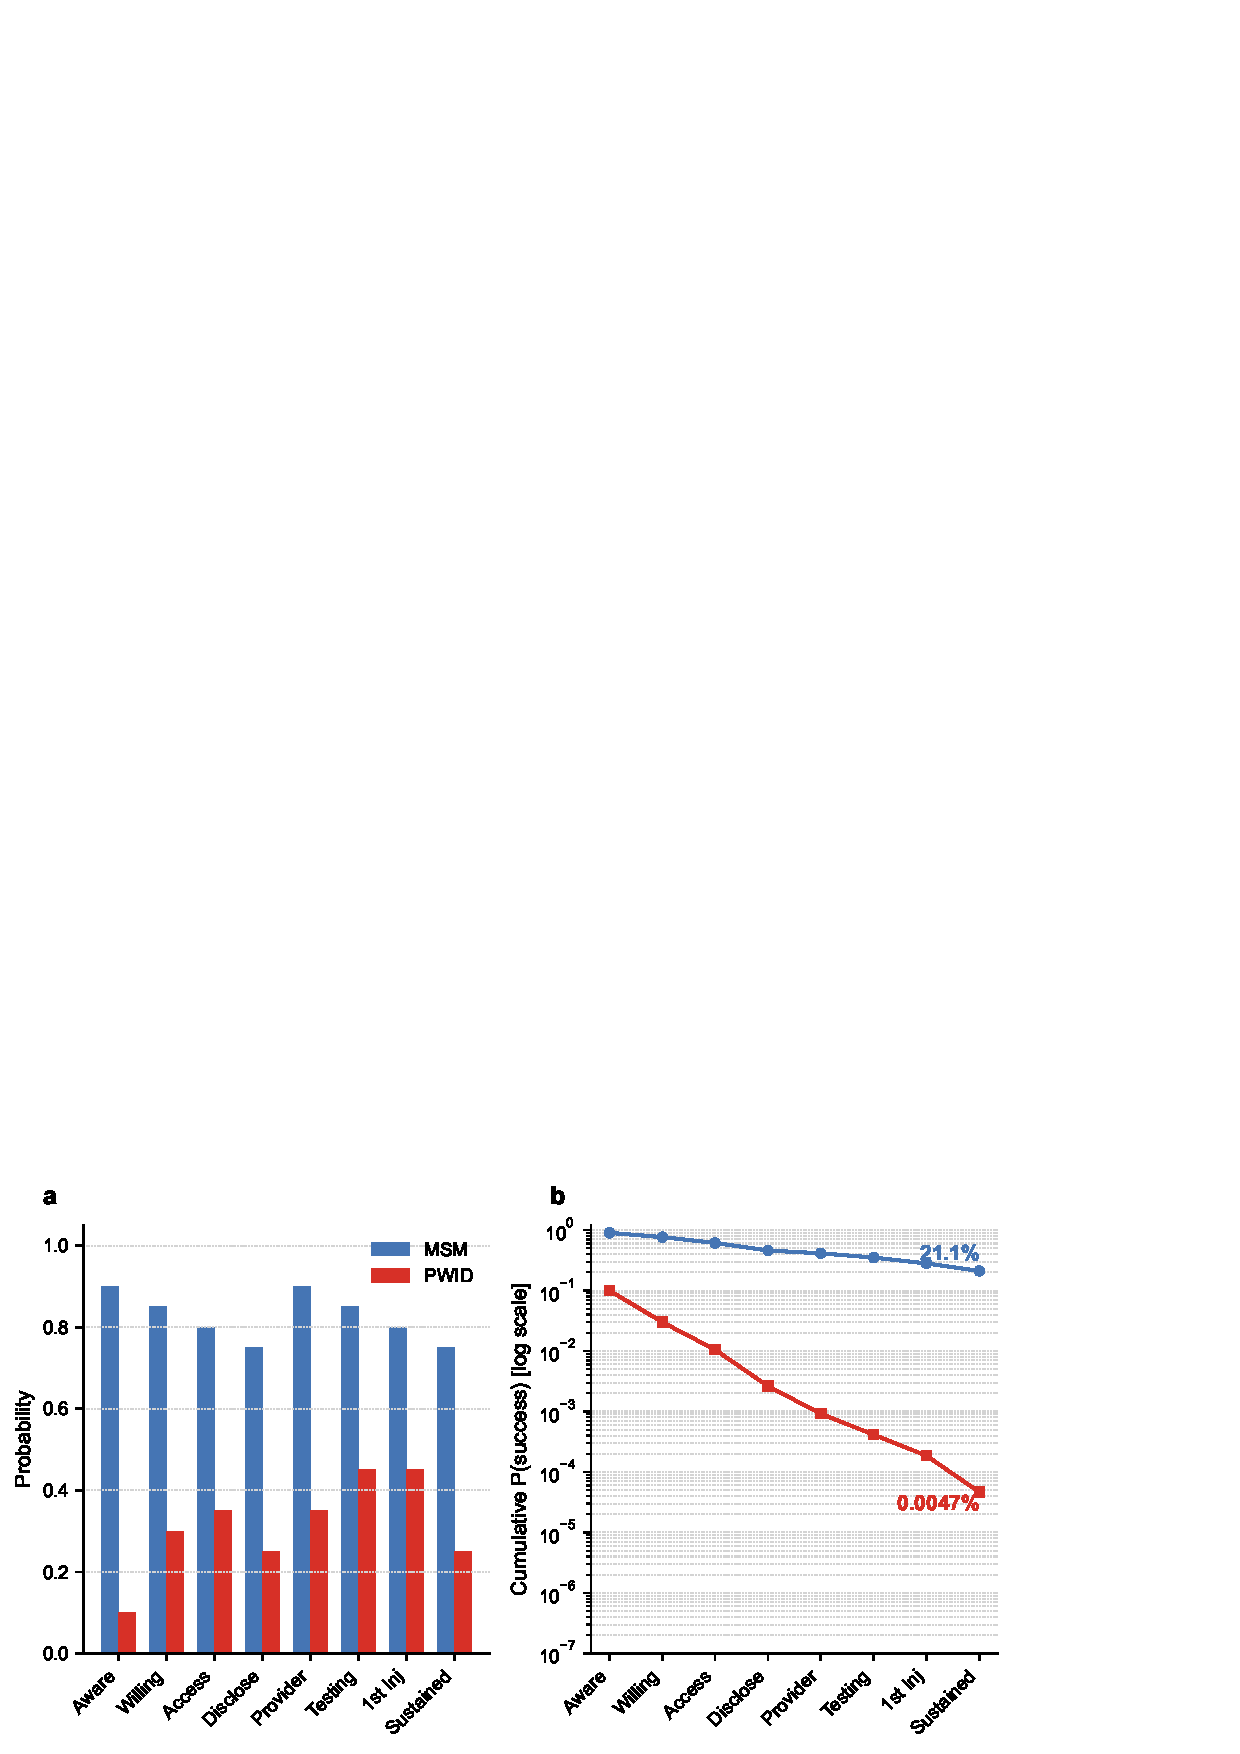
\includegraphics[width=\textwidth]{Fig1_CascadeComparison.png}
\caption{\textbf{LAI-PrEP Cascade Comparison: MSM vs PWID.} Step-wise probabilities showing barrier-adjusted probability of completing each cascade step, demonstrating the dramatic disparity between MSM (cascade completion 21.1\%) and PWID (cascade completion 0.0047\%). Under current policy, 90\% of PWID fail at the awareness step.}
\label{fig:cascade}
\end{figure}

\subsection{Three-Layer Barrier Decomposition}

Barrier decomposition attributed failures as follows: Layer 1 (Pathogen Biology) 0.0\%, Layer 2 (HIV Testing) 6.8\%, and Layer 3 (Architectural Failures) 93.2\% (Figure 2). Within architectural failures, policy barriers (criminalization and incarceration) contributed 38.4\%, infrastructure barriers (MSM-centric design) 21.9\%, stigma barriers (healthcare discrimination) 20.5\%, machine learning barriers (algorithmic deprioritization) 8.2\%, and research exclusion barriers 4.1\%.

Notably, pathogen biology contributed 0.0\% to prevention failure because cascade attrition was so severe that very few individuals reached the point where pathogen dynamics became relevant. The irreversibility of HIV integration within hours remains fundamental to the requirement for \Rzero{}=0, but this biological constraint is never tested when 90\% fail at awareness.

\begin{figure}[ht]
\centering
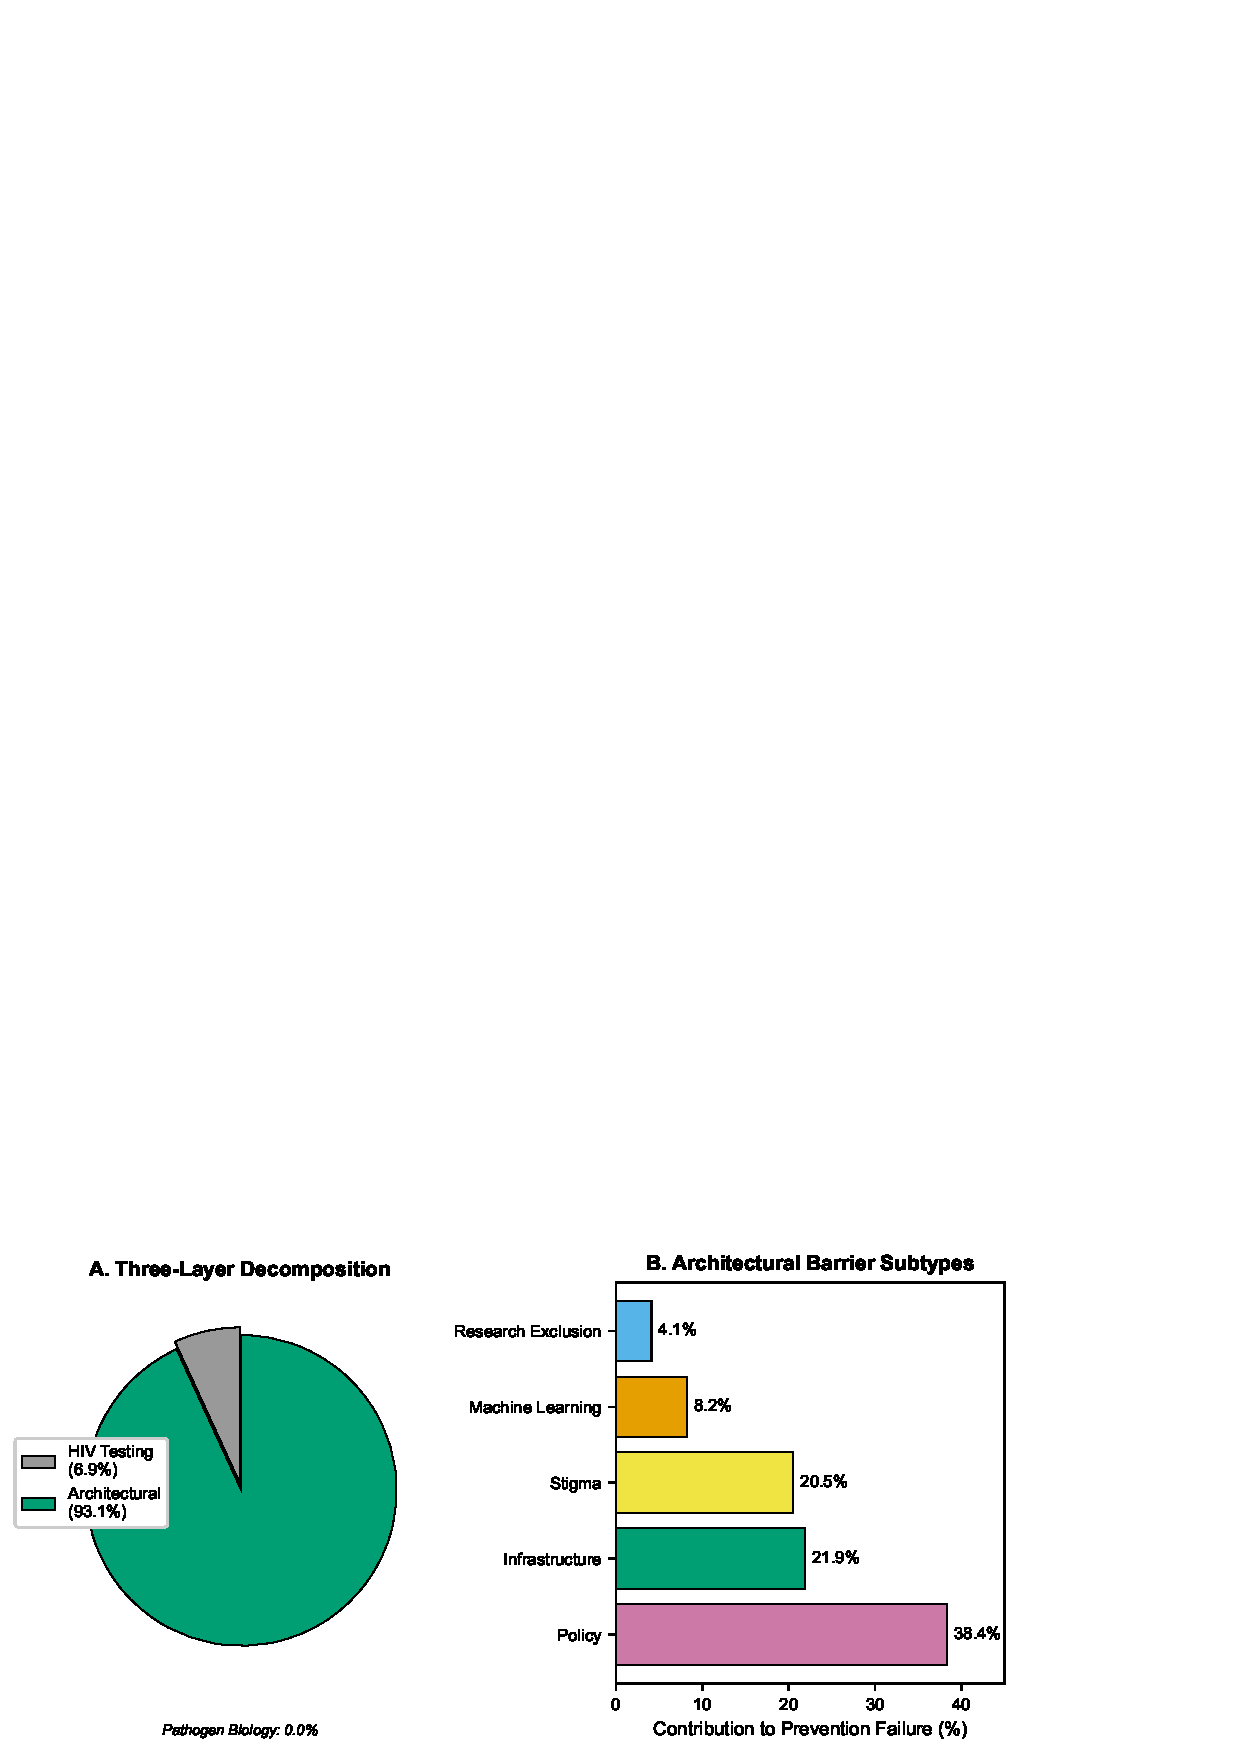
\includegraphics[width=\textwidth]{Fig2_BarrierDecomposition.png}
\caption{\textbf{Three-Layer Barrier Decomposition.} Distribution of prevention failure across three layers: Pathogen Biology (0.0\%), HIV Testing (6.8\%), and Architectural Failures (93.2\%). Within architectural failures: Policy (38.4\%), Infrastructure (21.9\%), Stigma (20.5\%), Machine Learning (8.2\%), and Research Exclusion (4.1\%).}
\label{fig:barriers}
\end{figure}

\subsection{Policy Scenario Analysis}

Table 1 presents P(\Rzero{}=0) across eight policy scenarios. Decriminalization alone increased P(\Rzero{}=0) from 0.00\% to 0.14\% (95\% CI: 0.12--0.17). Adding stigma reduction achieved 0.44\% (95\% CI: 0.40--0.48). SSP-integrated delivery with peer navigation reached 5.03\% (95\% CI: 4.89--5.16). Full harm reduction (SSP + OAT + housing + employment) achieved 9.42\% (95\% CI: 9.24--9.60). Incorporating PURPOSE-4 trial data (if PWID were included) increased this to 11.86\% (95\% CI: 11.66--12.06). Full harm reduction with algorithmic debiasing reached 18.62\% (95\% CI: 18.38--18.86). Theoretical maximum (all barriers removed) achieved 19.92\% (95\% CI: 19.67--20.17).

\begin{figure}[ht]
\centering
\includegraphics[width=\textwidth]{Fig3_PolicyScenarios.png}
\caption{\textbf{Policy Scenario Analysis.} P(\Rzero{}=0) across eight policy scenarios ranging from Current Policy (0.00\%) to Theoretical Maximum (19.92\%), with MSM comparison (16.30\%) shown for reference. SSP-integrated delivery achieves 5.03\%; full harm reduction achieves 9.42\%; algorithmic debiasing adds 9.20 percentage points.}
\label{fig:policy}
\end{figure}

\subsection{MSM vs PWID Disparity}

The MSM population receiving identical LAI-PrEP intervention achieved P(\Rzero{}=0) of 16.30\% compared to 0.00\% for PWID---an infinite-fold disparity. This difference emerged entirely from structural factors: MSM cascade step probabilities ranged from 75--95\% compared to 10--45\% for PWID. MSM incarceration survival over 5 years was 77.4\% compared to 16.8\% for PWID. The 120-fold disparity in signal-to-noise ratio (SNR) for machine learning training data (MSM: 9,180 publications; PWID: 76.4) contributed to algorithmic deprioritization that compounds other barriers (Figure 5).

\begin{figure}[ht]
\centering
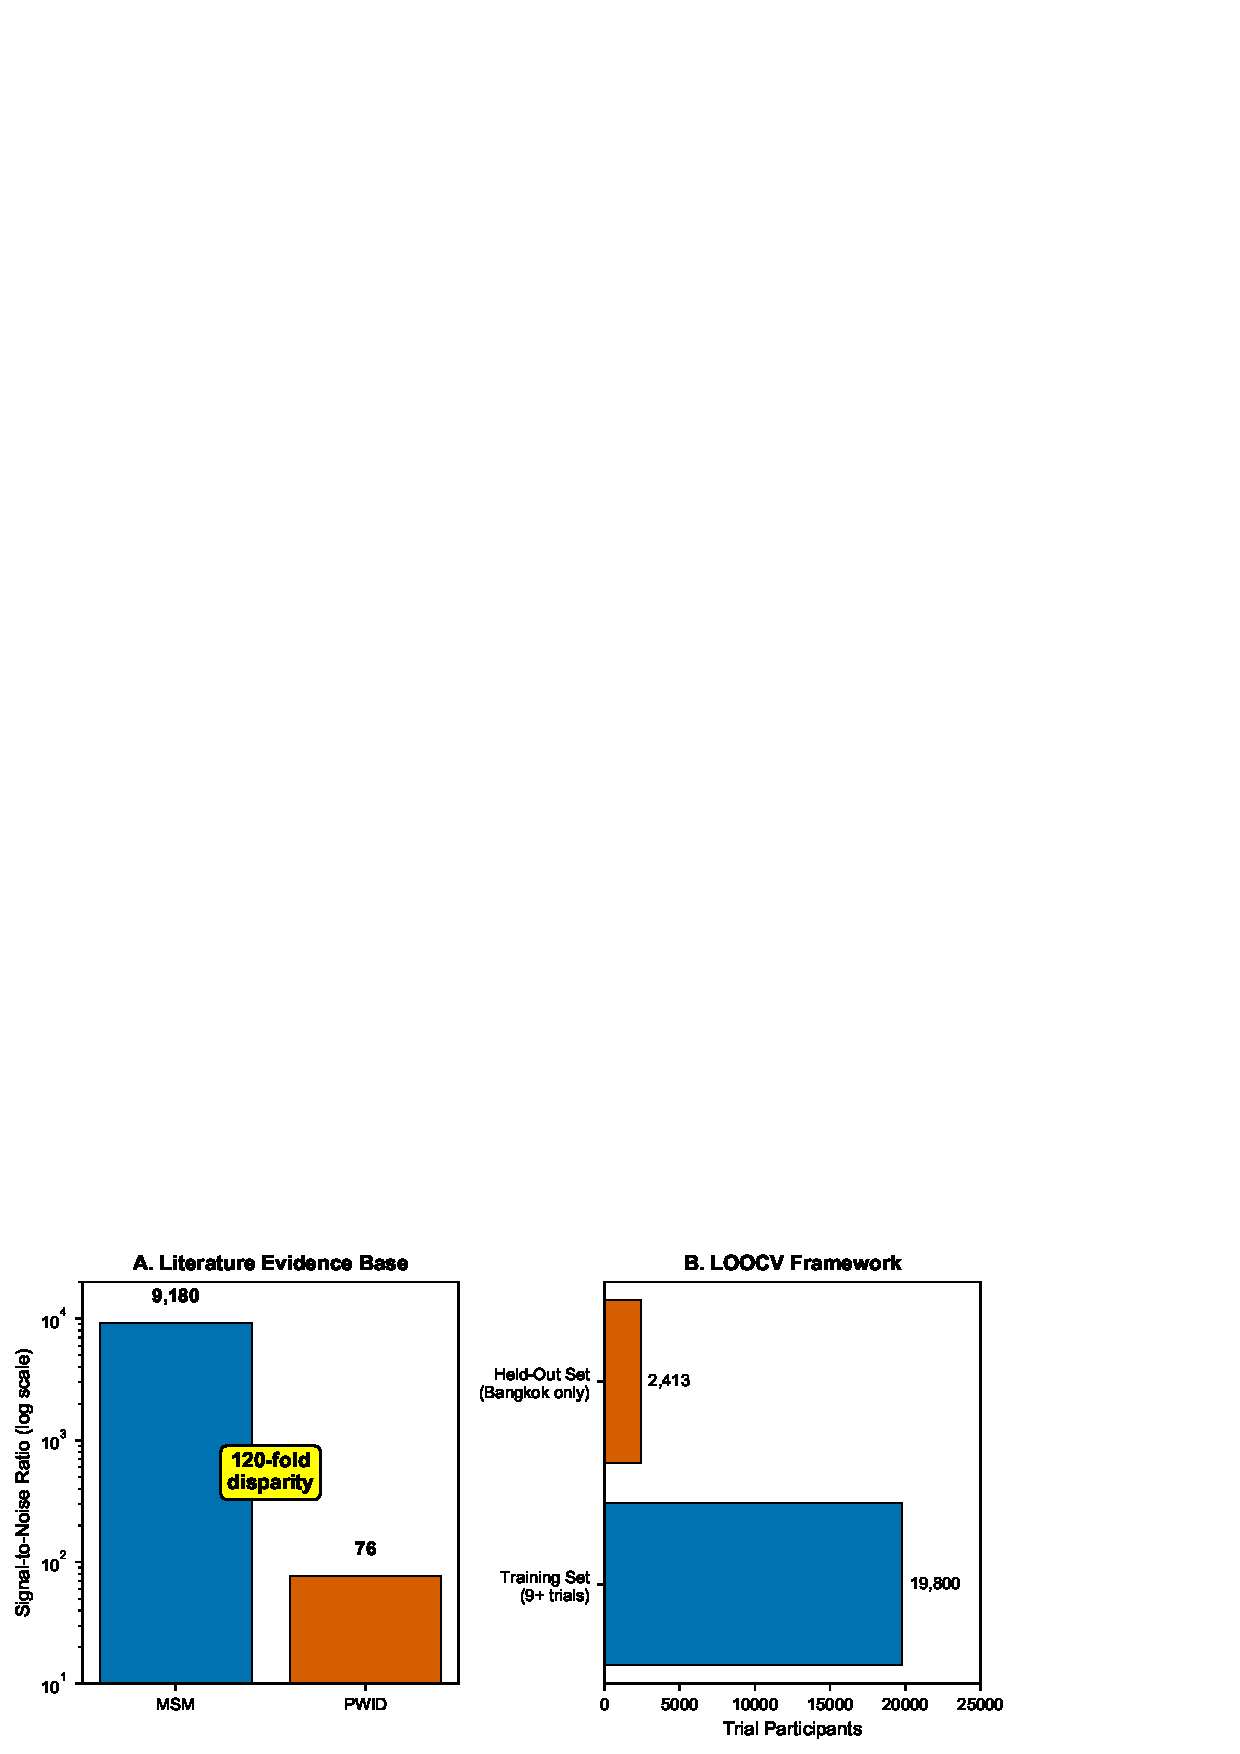
\includegraphics[width=\textwidth]{Fig5_SNR_LOOCV.png}
\caption{\textbf{Signal-to-Noise Ratio Disparity and LOOCV Framework.} Comparison of literature volume supporting machine learning algorithms: MSM (9,180 publications) vs PWID (76.4 publications, estimated)---a 120-fold disparity. The LOOCV framework shows systematic exclusion of PWID from HIV prevention trial evidence base, with PWID functioning as the ``held-out test population'' that was never validated.}
\label{fig:snr}
\end{figure}

\subsection{Stochastic Avoidance Failure Prediction}

The stochastic avoidance model predicted 63.3\% probability of major outbreak within 5 years under current conditions (Figure 4). Median time to outbreak was 4.0 years. Cumulative probability reached 87.6\% by 10 years. Network density trajectory showed progression from 0.895 (2024) toward the critical threshold, driven by methamphetamine prevalence growth.

Regional variation was substantial (Table 2): Pacific Northwest (baseline methamphetamine 35\%) showed 88\% 5-year outbreak probability with median 1.0 year; Appalachia (25\% baseline, 4\%/year growth) showed 78\% with median 2.0 years; Northeast Urban (12\% baseline, 5\%/year growth) showed 64\% with median 3.0 years; National Average showed 59\% with median 4.0 years.

\begin{figure}[ht]
\centering
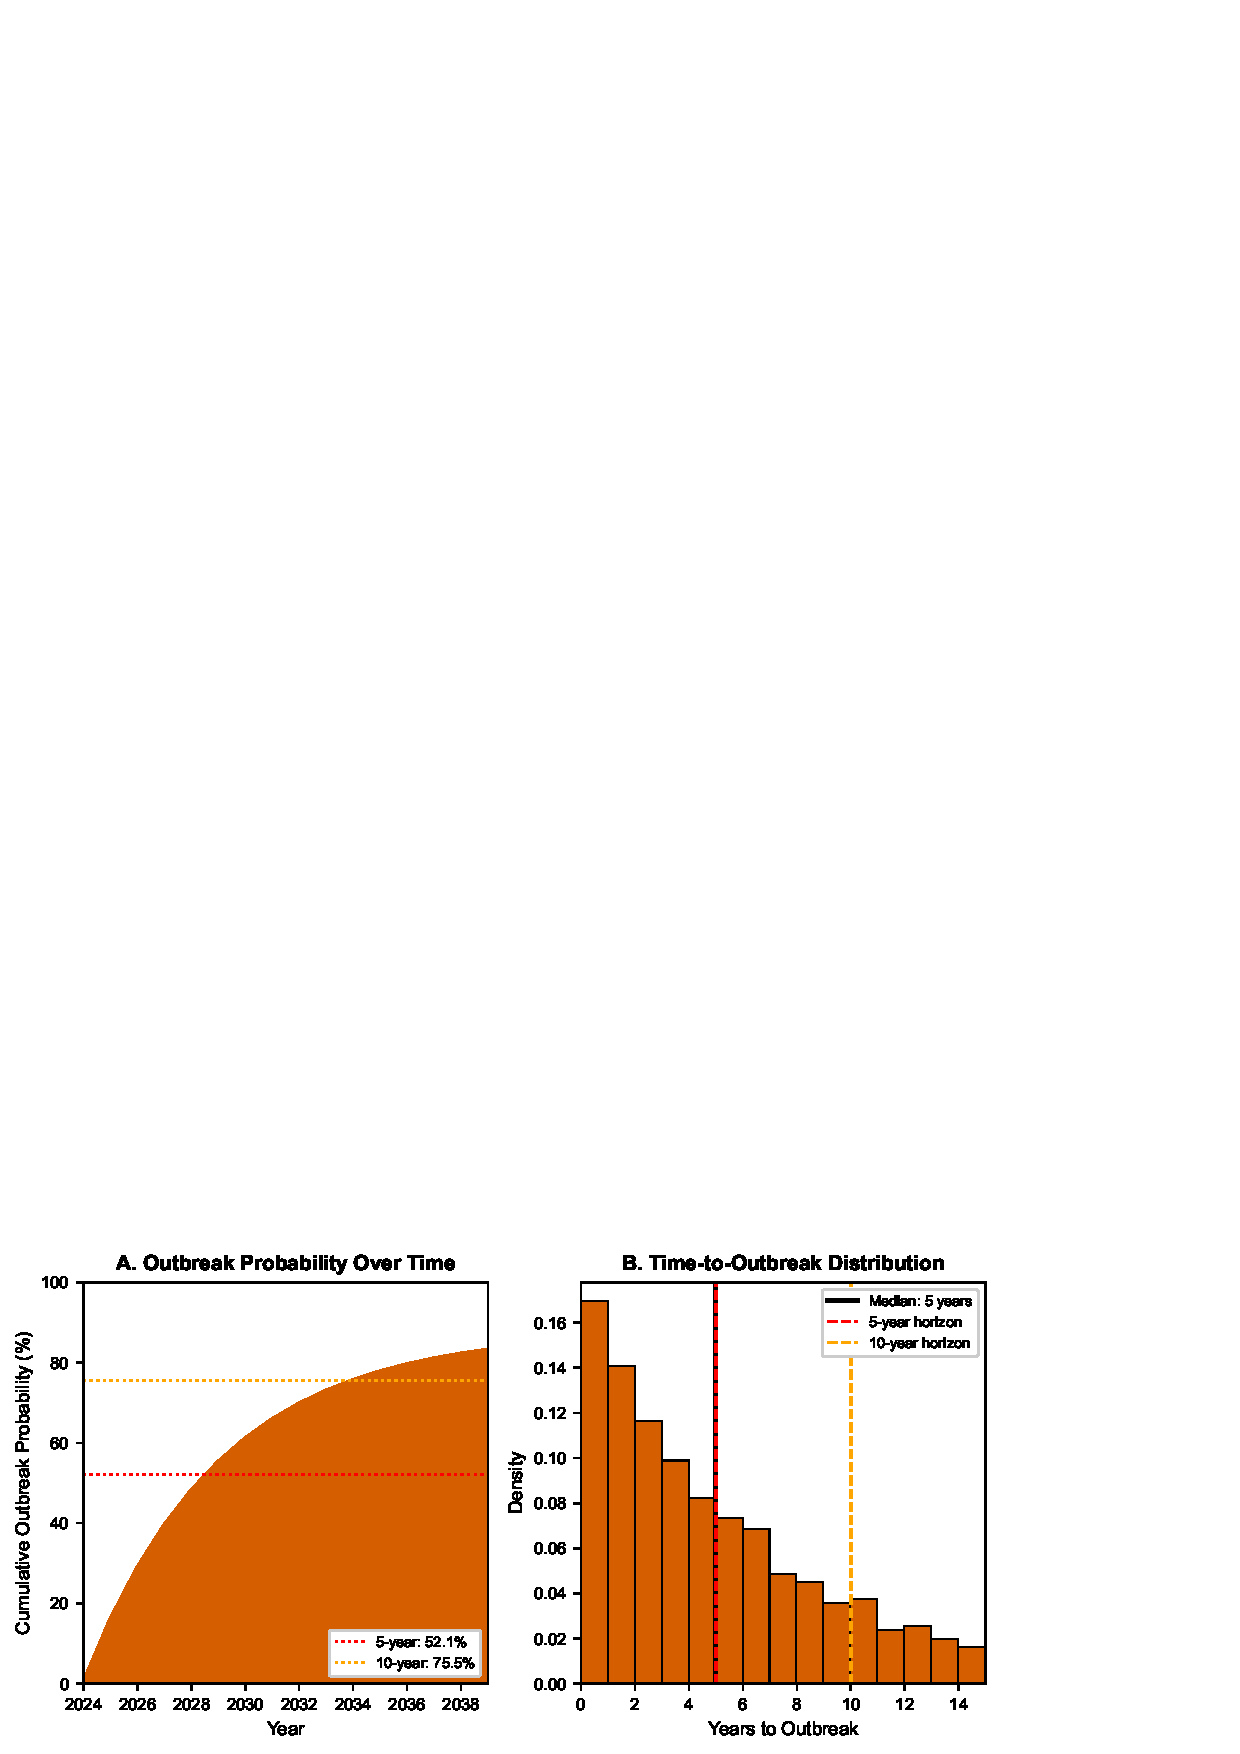
\includegraphics[width=\textwidth]{Fig4_StochasticAvoidance.png}
\caption{\textbf{Stochastic Avoidance Failure Prediction.} Cumulative outbreak probability over time with 90\% confidence interval, showing 63.3\% probability by 5 years and 87.6\% by 10 years. Time-to-outbreak distribution shows median 4.0 years with 80\% credible interval.}
\label{fig:stochastic}
\end{figure}

\subsection{Sensitivity Analysis}

Probabilistic sensitivity analysis confirmed robustness: mean P(\Rzero{}=0) under parameter uncertainty was 0.0005\% with 90\% CI (0.00\%, 0.00\%). Tornado analysis identified baseline outbreak probability ($\pm$49.8 percentage points), critical network threshold ($\pm$17.8pp), and methamphetamine network multiplier ($\pm$16.6pp) as most influential parameters. Barrier removal analysis showed that eliminating criminalization alone increased P(\Rzero{}=0) from 0.00\% to 0.23\%; removing all architectural barriers achieved 19.88\%.

% DISCUSSION
\section{Discussion}

This analysis demonstrates that HIV prevention failure among PWID results from policy-determined structural barriers, not pharmacological limitations or individual behavior. The same LAI-PrEP intervention achieving 16.30\% sustained protection among MSM achieves 0.00\% among PWID---a disparity that cannot be explained by drug efficacy, which is identical. Rather, nested barriers operating at the architectural level create conditions where the mathematical requirement for epidemic control (\Rzero{}=0) is unachievable.

The three-layer barrier framework reveals that pathogen biology contributes 0.0\% to current prevention failure---not because viral dynamics are irrelevant, but because cascade attrition is so severe that HIV's biological constraints are never tested. When 90\% of PWID fail at the awareness step,\cite{biello_prep_2018,mistler_prep_2021} the 4--72 hour window for prevention becomes meaningless. This finding fundamentally reframes the prevention challenge: we do not need better drugs; we need policy change that allows existing drugs to reach their intended recipients.

The concept of stochastic avoidance provides critical context for understanding why catastrophic outbreaks among PWID remain sporadic despite systematic prevention failure. HIV transmission requires the intersection of an infected person, a susceptible person, and a transmission event---conditions that may fail to occur simultaneously by chance alone.\cite{greenhalgh_stochastic_2016} Des Jarlais and colleagues demonstrated that even with 10--20\% syringe sharing rates, HIV can remain at low prevalence through ``firewall effects'' where infected individuals in low-infectiousness states block transmission to network segments.\cite{desjarlais_hiv_2016,bobashev_firewall_2013} This stochastic protection, however, is inherently unstable and time-limited.

Methamphetamine introduction into PWID communities represents a critical threat to stochastic avoidance.\cite{glick_meth_2018,strathdee_meth_2014} With hazard ratios of 1.46--7.11 for HIV seroconversion,\cite{plankey_meth_2007,grov_meth_2020} methamphetamine increases both transmission probability and network connectivity through hypersexuality, increased injection frequency, and bridging between MSM and non-MSM PWID networks. Our model predicts 63\% probability of major outbreak within 5 years under current conditions, with regional variation reflecting differential methamphetamine penetration.

The systematic exclusion of PWID from HIV prevention research compounds these barriers.\cite{brody_exclusion_2021,kamitani_bestpractices_2024} While the Bangkok Tenofovir Study demonstrated 48.9\% efficacy among PWID in 2013,\cite{choopanya_bangkok_2013} no major LAI-PrEP trial has enrolled this population. HPTN 083 and 084 explicitly excluded injection drug use; PURPOSE-2 enrolled cisgender women but not PWID.\cite{kelley_purpose2_2024} Meanwhile, hepatitis C trials have successfully enrolled and retained active PWID with 94--97\% treatment completion rates\cite{grebely_simplify_2018,dore_cedge_2016}---demonstrating that research engagement is feasible when investigators choose to include this population.

This research exclusion has downstream effects through machine learning algorithms that increasingly guide clinical decision-making. With a 120-fold disparity in training data quality between MSM and PWID, algorithms trained on HIV prevention literature will systematically deprioritize PWID patients regardless of clinical indication. This represents a novel barrier type that amplifies existing disparities through ostensibly neutral technological systems.

\subsection{Limitations}

This analysis has several limitations. First, cascade parameters derive from heterogeneous literature sources with varying methodologies; we addressed this through sensitivity analysis demonstrating robustness. Second, the stochastic avoidance model simplifies complex network dynamics; actual outbreak timing will depend on local factors not captured in aggregate parameters. Third, policy scenarios represent idealized conditions; real-world implementation would involve partial and gradual changes. Fourth, we assumed barrier effects are multiplicative; synergistic or antagonistic interactions may exist. Despite these limitations, the fundamental finding---that P(\Rzero{}=0) approaches zero under current policy---appears robust across all sensitivity analyses.

\subsection{Implications for Policy and Practice}

Our findings indicate that no single intervention can achieve epidemic control among PWID. Even with full decriminalization, harm reduction infrastructure, and research inclusion, maximum achievable P(\Rzero{}=0) remains below 20\%. This reflects the multiplicative nature of cascade barriers: improving any single step yields minimal benefit when other steps remain at 25--45\% probability. Effective intervention requires simultaneous action across all barrier layers.

The 63\% five-year outbreak probability demands urgent action. Van Handel and colleagues identified 220 vulnerable U.S. counties in 2016,\cite{van_handel_vulnerability_2016} yet only 21\% had syringe services programs operating as of 2018. The outbreaks in Scott County,\cite{peters_scottcounty_2016,gonsalves_scottcounty_2018} Lawrence/Lowell,\cite{alpren_massachusetts_2020} and Cabell/Kanawha Counties\cite{mcclung_cabell_2021,bonacci_kanawha_2023} occurred precisely where stochastic protection failed in the absence of systematic intervention. These were not unpredictable events; they were probabilistically inevitable consequences of policy choices.

\section{Conclusions}

HIV prevention among PWID exists in a state of manufactured death---conditions created by policy that render epidemic control mathematically impossible regardless of pharmacological innovation. The same drugs achieving 16.30\% sustained protection in MSM achieve 0.00\% in PWID, not because of biological differences, but because of structural barriers functioning as exclusion criteria. Current prevention relies on stochastic avoidance, a time-limited phenomenon predicted to fail catastrophically within 4--5 years median.

Achieving epidemic control requires fundamental policy change: decriminalization of drug use, elimination of healthcare stigma, redesign of prevention infrastructure to include PWID, mandatory inclusion in clinical trials, and algorithmic debiasing of clinical decision support systems. Without such changes, future outbreaks are not possibilities---they are certainties. The question is not whether stochastic avoidance will fail, but when.

\section*{Data Sharing}

All model code, simulation outputs, and analysis scripts are available at \url{https://github.com/Nyx-Dynamics/hiv-prevention-master}. All model inputs derive from published literature or synthetic populations requiring no individual-level data privacy protections.

\section*{Declaration of Interests}

The author declares no competing interests.

\section*{Acknowledgments}

The author thanks the HIV prevention research community whose published work provided model parameters, and the PWID community advocates whose testimony informed barrier characterization.

\section*{Author Contributions}

ACD conceived the study, developed the theoretical framework, conducted the literature synthesis, built the computational models, performed all analyses, and wrote the manuscript.

\newpage

% TABLES

\begin{table}[ht]
\caption{P(\Rzero{}=0) by Policy Scenario (n=100,000 per scenario)}
\centering
\begin{tabular}{lccc}
\toprule
\textbf{Scenario} & \textbf{P(\Rzero{}=0)} & \textbf{95\% CI} & \textbf{Cascade \%} \\
\midrule
Current Policy & 0.00\% & (0.00, 0.00) & 0.01\% \\
Decriminalization Only & 0.14\% & (0.12, 0.17) & 0.23\% \\
Decrim + Stigma Reduction & 0.44\% & (0.40, 0.48) & 0.72\% \\
SSP-Integrated Delivery & 5.03\% & (4.89, 5.16) & 8.12\% \\
Full Harm Reduction & 9.42\% & (9.24, 9.60) & 9.42\% \\
Full HR + PURPOSE-4 Data & 11.86\% & (11.66, 12.06) & 11.86\% \\
Full HR + ML Debiasing & 18.62\% & (18.38, 18.86) & 18.62\% \\
Theoretical Maximum & 19.92\% & (19.67, 20.17) & 19.92\% \\
\midrule
\textbf{MSM (Comparison)} & \textbf{16.30\%} & --- & \textbf{21.07\%} \\
\bottomrule
\end{tabular}
\label{tab:scenarios}

\small\textit{Note:} MSM comparison represents identical pharmacological intervention with dramatically different structural context. Disparity is policy-determined, not pharmacology-determined.
\end{table}

\begin{table}[ht]
\caption{Regional Outbreak Probability Predictions}
\centering
\begin{tabular}{lccc}
\toprule
\textbf{Region} & \textbf{P(5 years)} & \textbf{P(10 years)} & \textbf{Meth Baseline (2018)} \\
\midrule
National Average & 59\% & 85\% & 14.3\% \\
Appalachia & 78\% & 94\% & 25\% \\
Pacific Northwest & 88\% & 98\% & 35\% \\
Northeast Urban & 64\% & 89\% & 12\% (5\%/yr growth) \\
\bottomrule
\end{tabular}
\label{tab:regional}
\end{table}

\newpage

% FIGURE LEGENDS

\section*{Figure Legends}

\textbf{Figure 1.} LAI-PrEP Cascade Comparison: MSM vs PWID. (A) Step-wise probabilities showing barrier-adjusted probability of completing each cascade step. (B) Cumulative cascade attrition on logarithmic scale, demonstrating 4,500-fold disparity in cascade completion (MSM 21.1\% vs PWID 0.0047\%). Under current policy, 90\% of PWID fail at the awareness step.

\textbf{Figure 2.} Three-Layer Barrier Decomposition. (A) Distribution of prevention failure across three layers: Pathogen Biology (0.0\%), HIV Testing (6.8\%), and Architectural Failures (93.2\%). (B) Decomposition of architectural failures into five subtypes: Policy (38.4\%), Infrastructure (21.9\%), Stigma (20.5\%), Machine Learning (8.2\%), and Research Exclusion (4.1\%).

\textbf{Figure 3.} Policy Scenario Analysis. P(\Rzero{}=0) across eight policy scenarios ranging from Current Policy (0.00\%) to Theoretical Maximum (19.92\%), with MSM comparison (16.30\%) shown for reference. SSP-integrated delivery with peer navigation achieves 5.03\%; full harm reduction achieves 9.42\%; algorithmic debiasing adds 9.20 percentage points.

\textbf{Figure 4.} Stochastic Avoidance Failure Prediction. (A) Cumulative outbreak probability over time with 90\% confidence interval, showing 63.3\% probability by 5 years and 87.6\% by 10 years. (B) Time-to-outbreak distribution showing median 4.0 years with 80\% credible interval.

\textbf{Figure 5.} Signal-to-Noise Ratio Disparity. (A) Comparison of literature volume supporting machine learning algorithms: MSM (9,180 publications) vs PWID (76.4 publications, estimated)---a 120-fold disparity. (B) LOOCV framework showing systematic exclusion of PWID from HIV prevention trial evidence base, with PWID functioning as the ``held-out test population'' that was never validated.

\newpage

% SUPPLEMENTARY FIGURES
\section*{Supplementary Figures}

\begin{figure}[ht]
\centering
\includegraphics[width=\textwidth]{FigS1_MethTrajectories.png}
\caption{\textbf{Supplementary Figure 1: Regional Methamphetamine Prevalence Trajectories.} (A) Projected methamphetamine-opioid co-use prevalence from 2018--2040 across seven U.S. regions. Pacific Northwest shows highest baseline (35\%), while Northeast Urban shows fastest growth (5\%/year). (B) Network density evolution with 90\% CI, showing approach toward critical threshold (0.35) that triggers exponential outbreak probability.}
\label{fig:s1}
\end{figure}

\begin{figure}[ht]
\centering
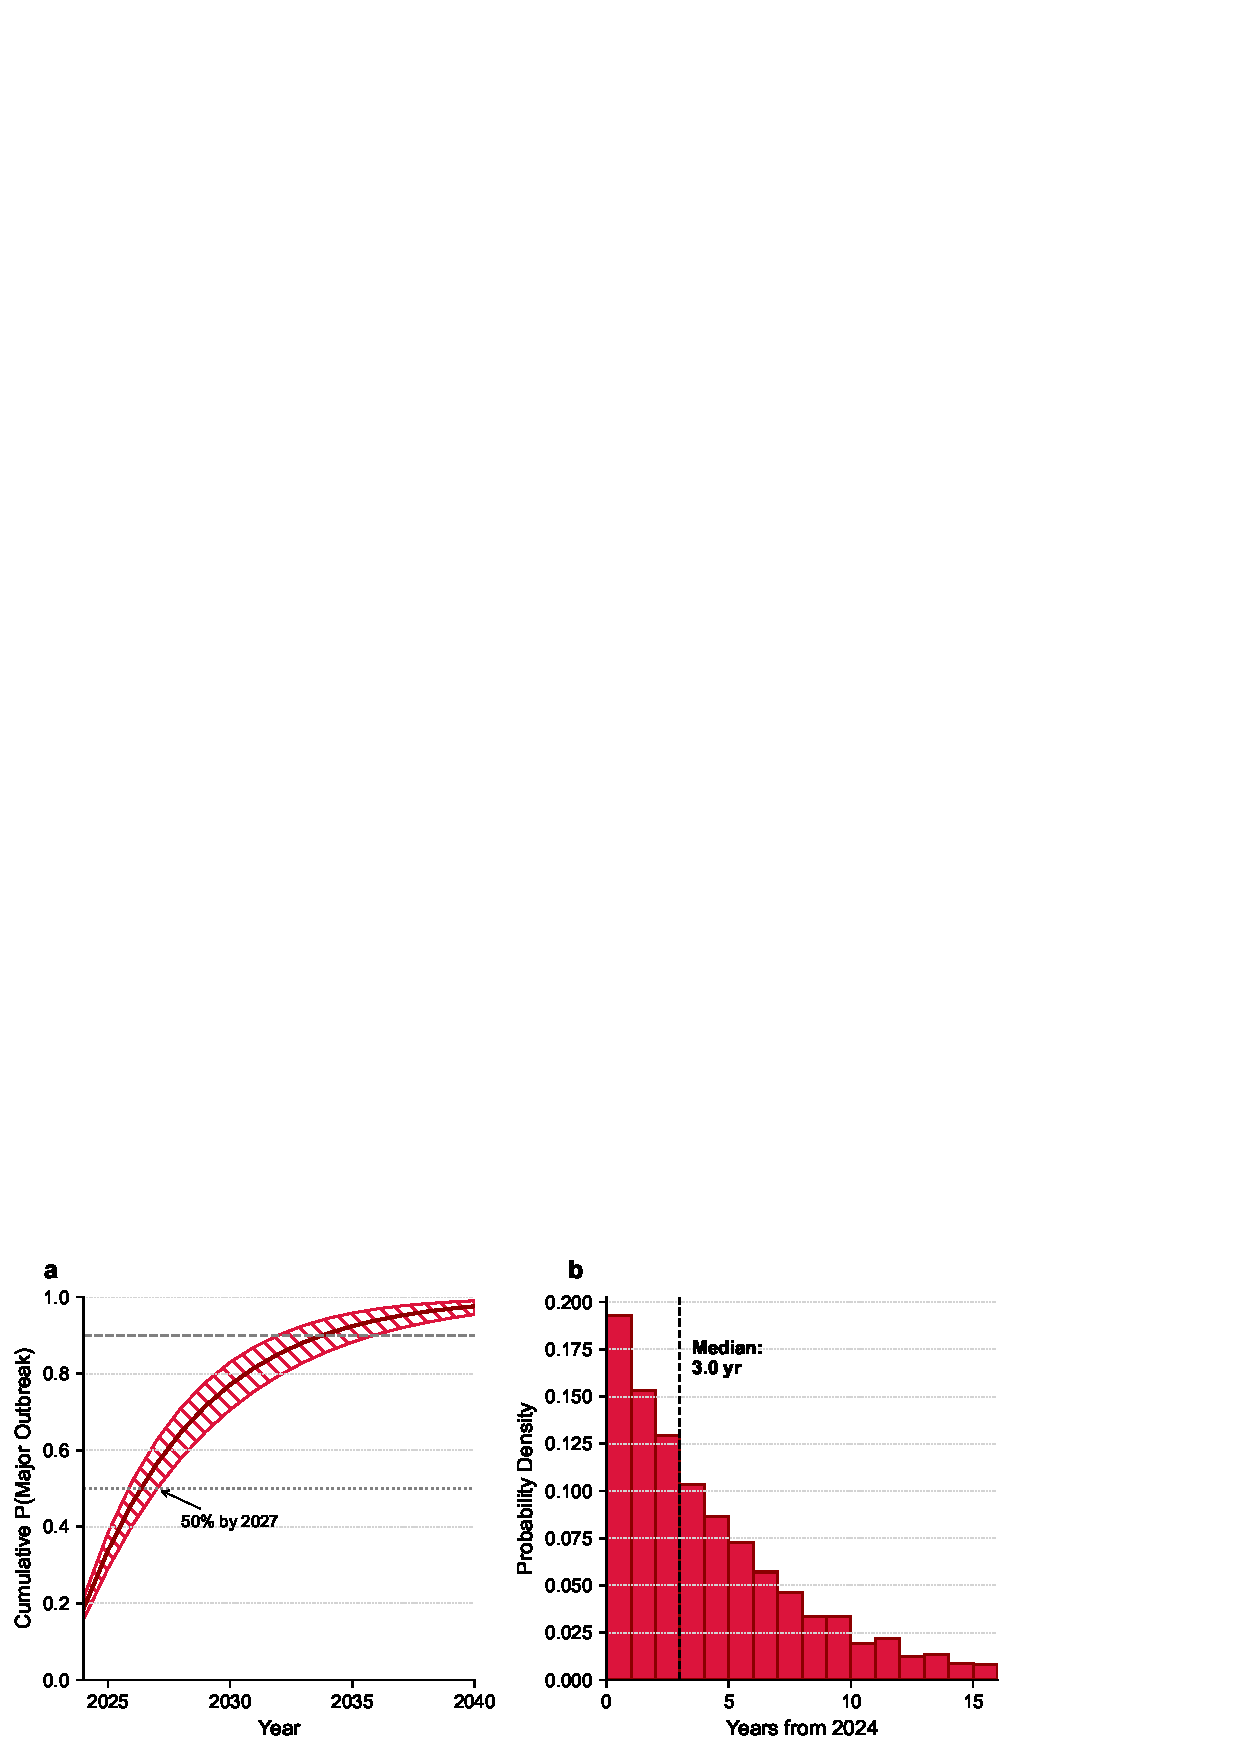
\includegraphics[width=\textwidth]{FigS2_OutbreakForecast.png}
\caption{\textbf{Supplementary Figure 2: Outbreak Probability Forecast.} (A) Cumulative outbreak probability 2024--2040 with 90\% confidence interval. Horizontal lines indicate 50\% and 90\% probability thresholds. (B) Time-to-outbreak distribution histogram with median (4.0 years) and 80\% credible interval marked.}
\label{fig:s2}
\end{figure}

\begin{figure}[ht]
\centering
\includegraphics[width=\textwidth]{FigS3_TornadoDiagram.png}
\caption{\textbf{Supplementary Figure 3: Tornado Diagram---Parameter Sensitivity.} Top 10 parameters ranked by impact on 5-year outbreak probability. Red bars indicate parameter values that increase outbreak risk; green bars indicate values that decrease risk. Baseline annual outbreak probability ($\pm$49.8pp) and critical network threshold ($\pm$17.8pp) are most influential.}
\label{fig:s3}
\end{figure}

\begin{figure}[ht]
\centering
\includegraphics[width=\textwidth]{FigS4_ScenarioComparison.png}
\caption{\textbf{Supplementary Figure 4: Policy Scenario Comparison.} (A) 5-year outbreak probability by intervention scenario, color-coded by risk level (red = high, yellow = moderate, green = low). (B) Median years to outbreak by scenario. Current policy: 57\% 5-year risk, 4.5 years median. Full harm reduction: 41\% 5-year risk, 7.0 years median.}
\label{fig:s4}
\end{figure}

\begin{figure}[ht]
\centering
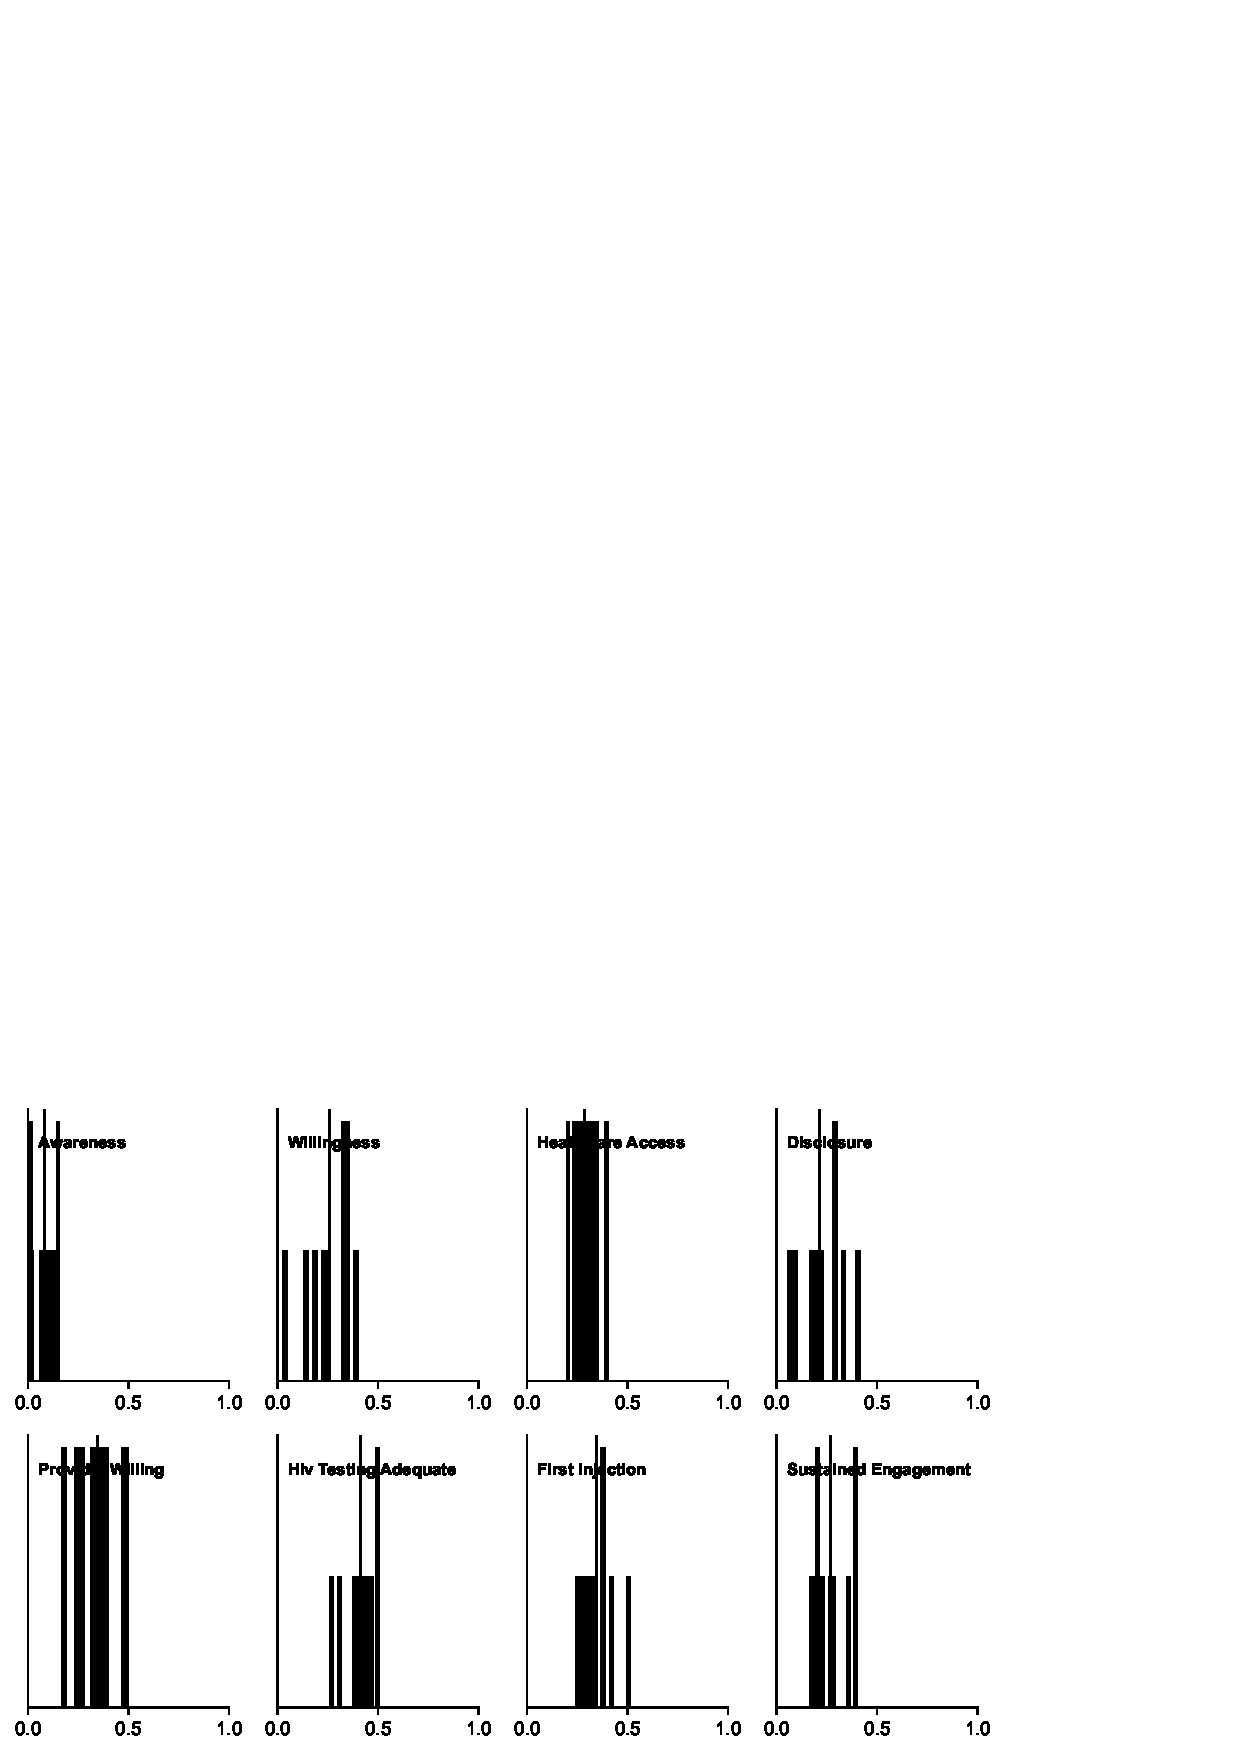
\includegraphics[width=\textwidth]{FigS5_CascadeUncertainty.png}
\caption{\textbf{Supplementary Figure 5: Cascade Step Probability Distributions Under Parameter Uncertainty.} Eight panels showing probability distributions for each cascade step from probabilistic sensitivity analysis (n=1,000 samples). Mean, 5th percentile, and 95th percentile marked for each step.}
\label{fig:s5}
\end{figure}

\begin{figure}[ht]
\centering
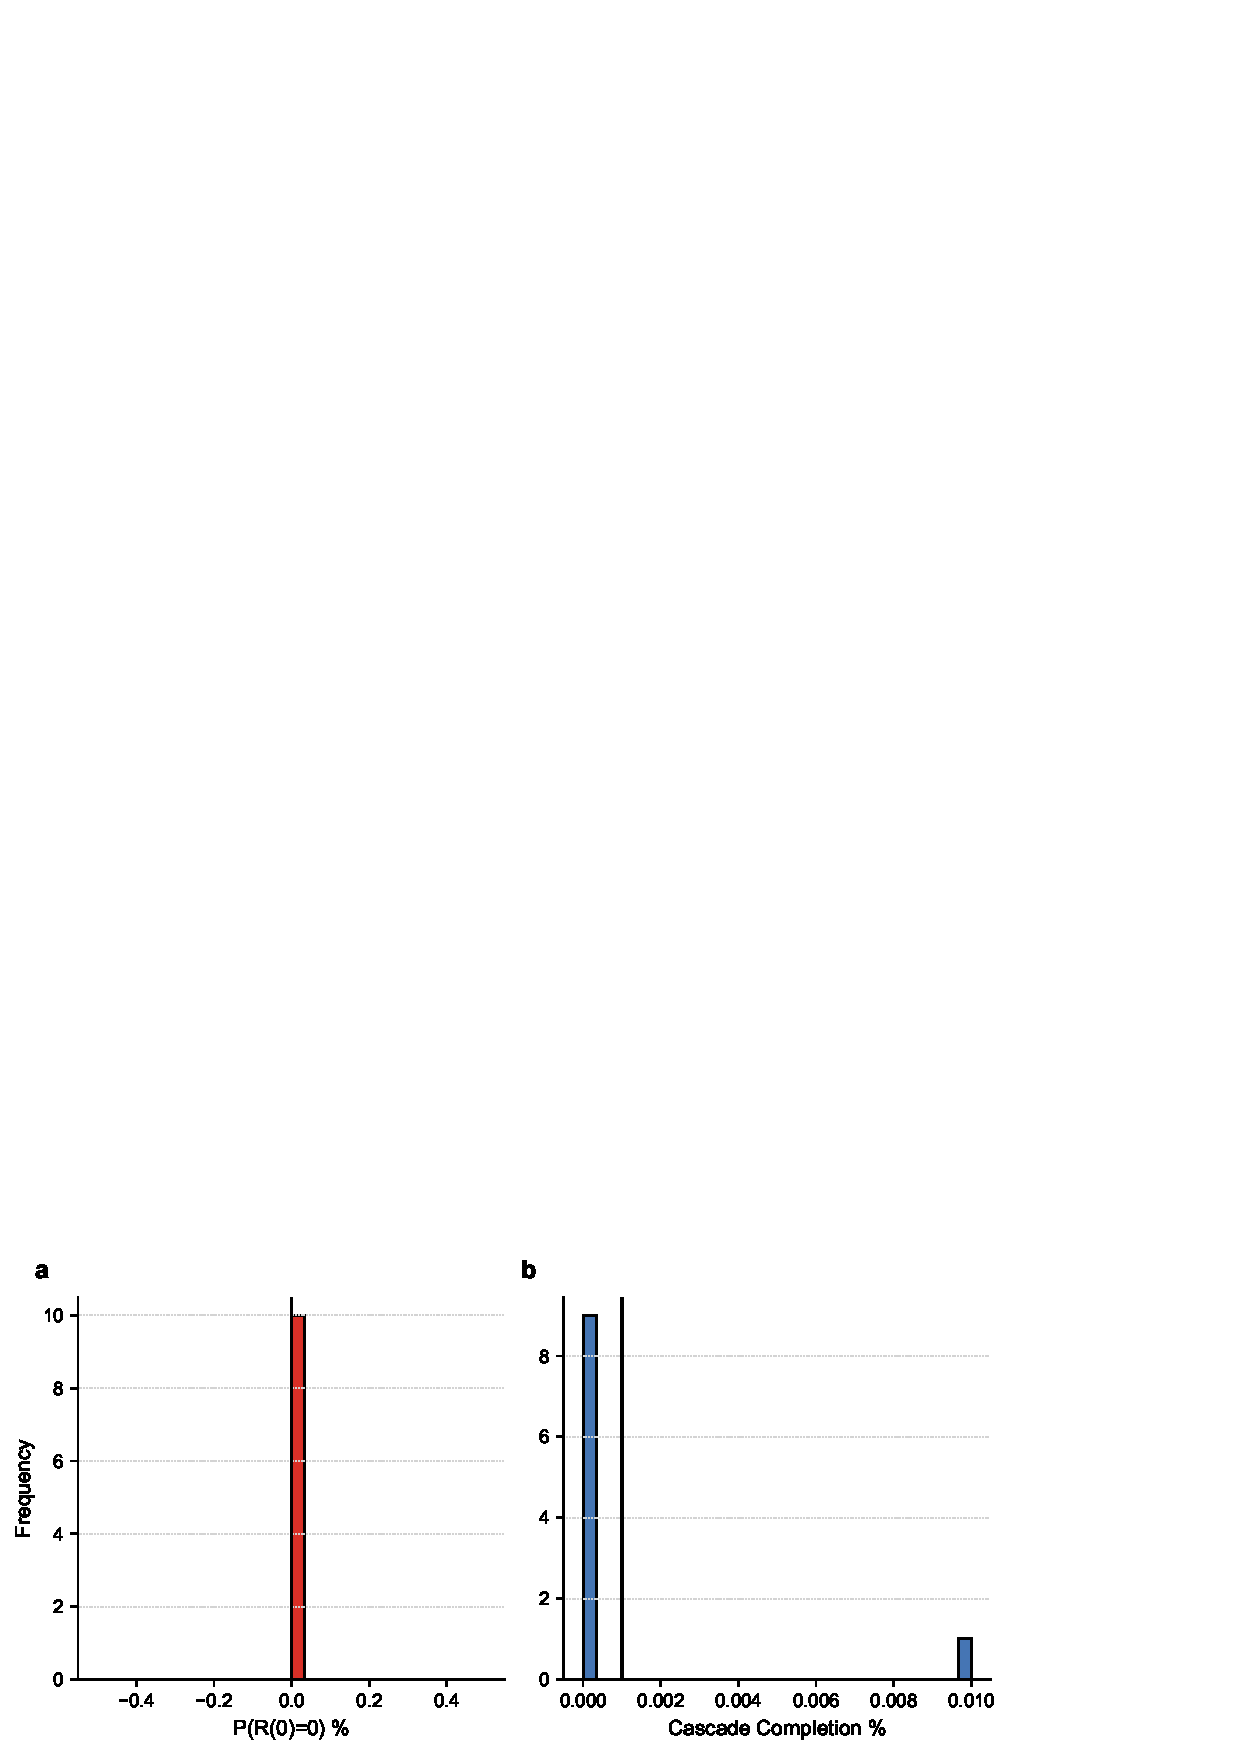
\includegraphics[width=\textwidth]{FigS6_R0ZeroDistribution.png}
\caption{\textbf{Supplementary Figure 6: P(\Rzero{}=0) Distribution from Probabilistic Sensitivity Analysis.} (A) Distribution of P(\Rzero{}=0) across 1,000 parameter samples, demonstrating robustness of finding (mean 0.0005\%, 90\% CI: 0.00--0.00\%). (B) Cascade completion distribution showing consistent near-zero completion rates regardless of parameter variation.}
\label{fig:s6}
\end{figure}

\begin{figure}[ht]
\centering
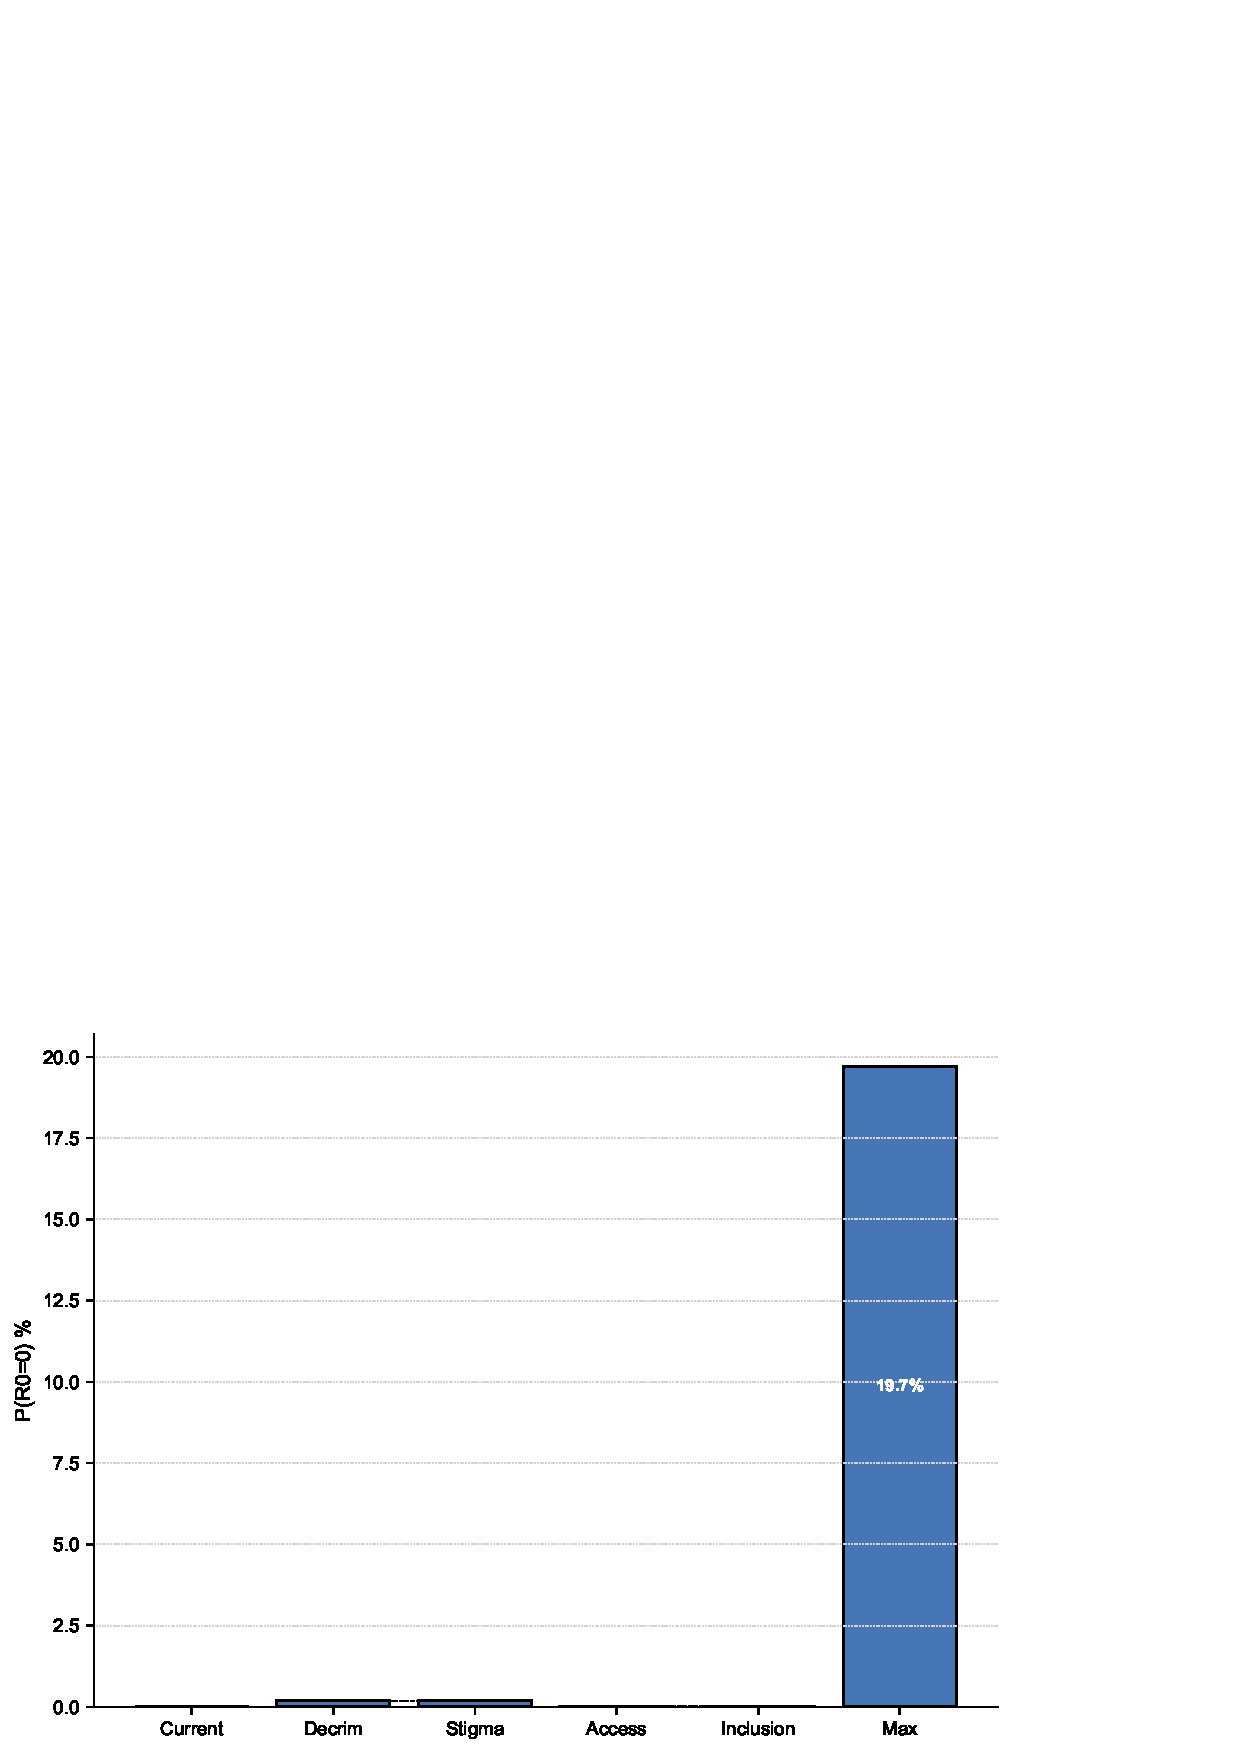
\includegraphics[width=\textwidth]{FigS7_BarrierRemoval.png}
\caption{\textbf{Supplementary Figure 7: Barrier Removal Waterfall Analysis.} Incremental effects of removing specific barrier types on P(\Rzero{}=0). Baseline (0.00\%) $\rightarrow$ No criminalization (+0.23pp) $\rightarrow$ No stigma (+0.01pp) $\rightarrow$ Low-barrier access (+0.02pp) $\rightarrow$ Full research inclusion (+0.004pp) $\rightarrow$ All barriers removed (19.88\%). Demonstrates multiplicative barrier interactions requiring comprehensive intervention.}
\label{fig:s7}
\end{figure}

\begin{figure}[ht]
\centering
\includegraphics[width=0.8\textwidth]{FigS8_StepImportance.png}
\caption{\textbf{Supplementary Figure 8: Cascade Step Importance Ranking.} (A) Current step probabilities under current policy, color-coded by severity. (B) Improvement in P(\Rzero{}=0) if each step were fixed to 99\% probability. Sustained engagement shows largest individual impact (+0.01pp), but no single step fix achieves epidemic control---demonstrating the multiplicative cascade requiring simultaneous intervention across all steps.}
\label{fig:s8}
\end{figure}

\newpage

% REFERENCES
\bibliographystyle{unsrtnat}
\bibliography{unified_MD}

\end{document}
